\subsection{混合增益--相位稳定性判据}
\begin{figure}
\centering
\begin{subfigure}{0.45\columnwidth}
  \centering
  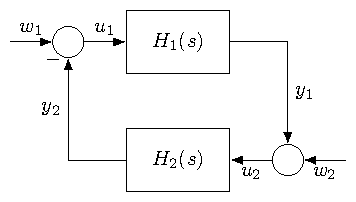
\includegraphics[width=\linewidth]{feedback_diagram.pdf}
  \caption{一般反馈系统。}
  \label{fig:fd_diagram}
\end{subfigure}
\begin{subfigure}{0.45\columnwidth}
  \centering
  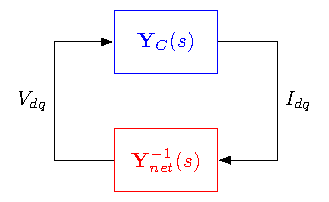
\includegraphics[width=\linewidth]{feedback_diagram_converters_2.pdf}
  \caption{导纳反馈。}
  \label{fig:fd_diagram_conv_net}
\end{subfigure}
\caption{反馈互连示意图。}
\label{fig:twoside}
\end{figure}

上述概念为评估线性时不变系统的稳定性提供了框架。考虑图~\ref{fig:fd_diagram} 所示 $H_1(s)$ 与 $H_2(s)$ 的反馈互连。下述定理给出了所得闭环系统稳定的一个充分条件~\cite{zhao2022smallgainmeetssmall}。

\begin{thm}[混合小增益--相位定理]
设开环系统 $H_1,H_2$ 为实、有理、稳定且真有理的传递函数矩阵。若对每个 $\omega\in[0,\infty]$，下列两项至少有一项成立，则闭环系统稳定：
\begin{enumerate}
\item 最大奇异值之积满足
\begin{equation*}
\overline{\sigma}(H_1(j\omega))\overline{\sigma}(H_2(j\omega))<1;
\end{equation*}
\item $H_1(j\omega)$ 为半扇形矩阵、$H_2(j\omega)$ 为扇形矩阵，且
\begin{equation*}
\overline{\phi}(H_1(j\omega))+\overline{\phi}(H_2(j\omega))<\pi,
\end{equation*}
\begin{equation*}
\underline{\phi}(H_1(j\omega))+\underline{\phi}(H_2(j\omega))>-\pi.
\end{equation*}
\end{enumerate}
\label{thm:mixed_small_gain_phase}
\end{thm}

该定理将传统小增益条件及其相位对应条件统一到同一个稳定性框架中。对每个频率，可以根据哪一种估计较不保守，选择基于增益或相位的界。

\subsection{电力系统稳定性的分散式条件}
\begin{figure}
\centering
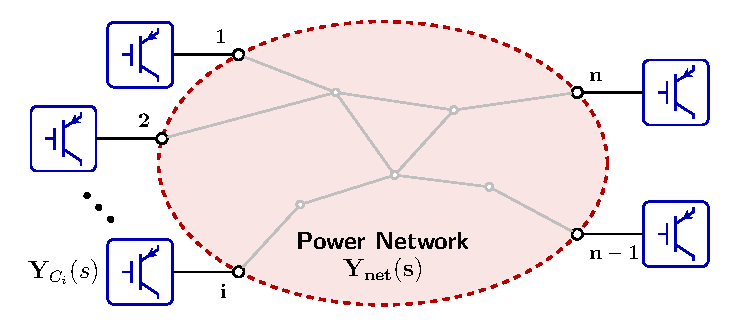
\includegraphics[width=\linewidth]{vsc1.pdf}
\caption{多变流器电力系统示意图。}
\label{fig:multi_converter_diagram}
\end{figure}

在电力系统中，我们关注图~\ref{fig:multi_converter_diagram} 所示 $n$ 台电力电子变流器接入给定网络后的互联系统稳定性。令
\begin{equation}
\mathbf{Y}_C(s)=\operatorname{diag}(Y_{C_1}(s),Y_{C_2}(s),\ldots,Y_{C_n}(s))
\label{eq:block_diagonal}
\end{equation}
表示总体变流器导纳矩阵，其中 $Y_{C_i}(s)$ 为第 $i$ 台变流器的导纳。令 $\mathbf{Y}_{net}(s)$ 表示网络导纳。本文假设 $\mathbf{Y}_{net}(s)$ 已经过 Kron 化简，即消除了所有未接入变流器的内部节点。所有导纳均表示在同一全局 $dq$ 坐标系中。与图~\ref{fig:fd_diagram} 类似，变流器和网络的互连可表示为图~\ref{fig:fd_diagram_conv_net} 所示反馈环路。

可以将定理~\ref{thm:mixed_small_gain_phase} 直接应用于该系统以获得稳定性条件。然而，$\mathbf{Y}_C(s)$ 的块对角结构允许开展分散式稳定性分析，从而得到下述结果~\cite{huangGainPhaseDecentralized2024}。

\begin{thm}[分散式混合小增益--相位定理]
若开环系统稳定，且对每个 $\omega\in[0,\infty]$，下列两项至少有一项成立，则图~\ref{fig:fd_diagram_conv_net} 所示多变流器系统稳定：
\begin{enumerate}
\item 分散式增益条件成立，即
\begin{equation*}
\max_i\overline{\sigma}(Y_{C_i}(j\omega))
<\underline{\sigma}(\mathbf{Y}_{net}(j\omega));
\end{equation*}
\item 分散式相位条件成立，即每个 $Y_{C_i}(j\omega)$ 均为拟扇形矩阵，$\mathbf{Y}_{net}(j\omega)$ 为扇形矩阵，并且
\begin{equation*}
\overline{\phi}(Y_{C_i}(j\omega))
<\pi-\overline{\phi}(\mathbf{Y}_{net}^{-1}(j\omega)),\quad\forall i,
\end{equation*}
\begin{equation*}
\underline{\phi}(Y_{C_i}(j\omega))
>-\pi-\underline{\phi}(\mathbf{Y}_{net}^{-1}(j\omega)),\quad\forall i,
\end{equation*}
\begin{equation*}
\max_i\overline{\phi}(Y_{C_i}(j\omega))
-\min_i\underline{\phi}(Y_{C_i}(j\omega))<\pi.
\end{equation*}
\end{enumerate}
\label{thm:dec_mixed_small_gain_phase}
\end{thm}

这种分散式表述只需检查每台变流器模型的局部条件以及网络模型的条件，便可认证大规模多变流器系统的稳定性，而无需显式计算完整互联系统的动态。
